\appendix
\section{Details}
\begin{itemize}
\item \cheng{Show the set of POI categories} \\
      Edinburgh: Cultural, Entertainment, Historical, Museum, Park, Structure \\
      Glasgow: Education, Museum, Park, Religion, Shopping, Structure, Transport \\
      Melbourne: City precincts, Entertainment, Institutions, Parks and spaces, Public galleries, Shopping, 
                 Sports stadiums, Structures, Transport \\
      Osaka: Amusement, Entertainment, Historical, Park \\
      Toronto: Amusement, Beach, Cultural, Shopping, Sport, Structure 
      The categories of POIs are shown in figure \ref{fig:poicats}.
      \begin{figure}
      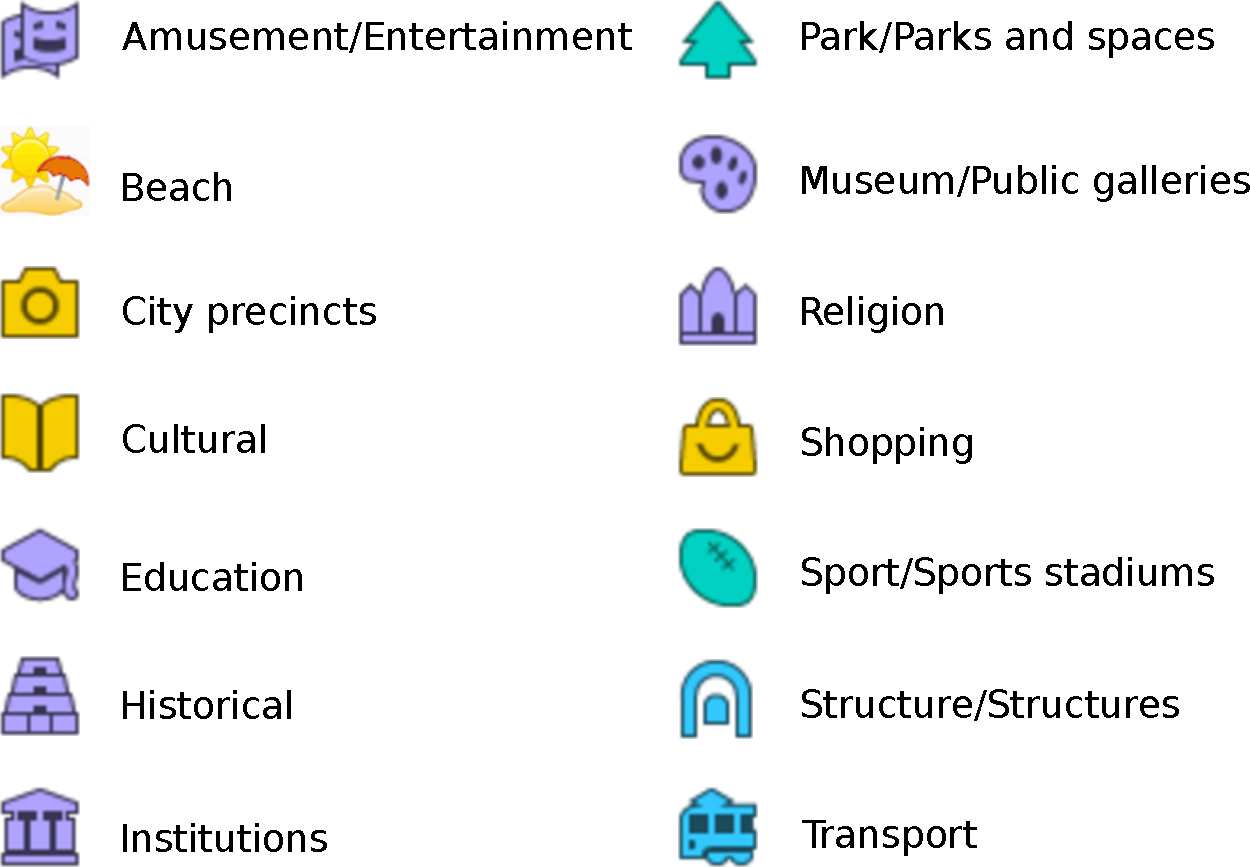
\includegraphics[width=\columnwidth]{fig/poi_cats.pdf}
      \caption{POI categories}
      \label{fig:poicats}
      \end{figure}
\item The distribution of POI popularity is shown in figure \ref{fig:popularity}.
      \begin{figure*}
      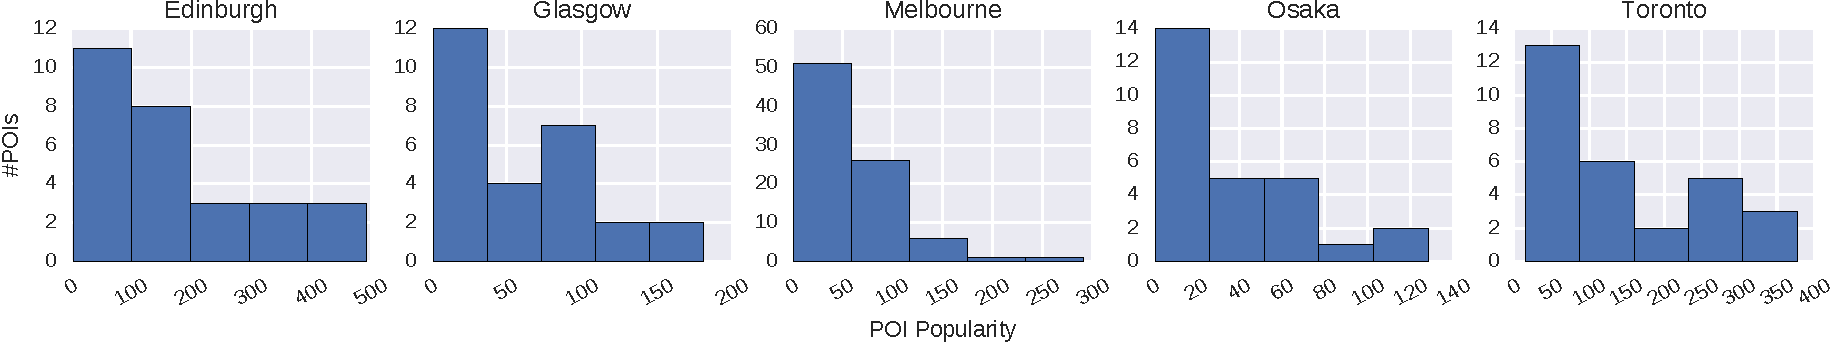
\includegraphics[width=\textwidth]{fig/poi_popularity.pdf}
      \caption{Distribution of POI popularity}
      \label{fig:popularity}
      \end{figure*}
\item The distribution of the number of visit at POI is shown in figure \ref{fig:nvisit}.
      \begin{figure*}
      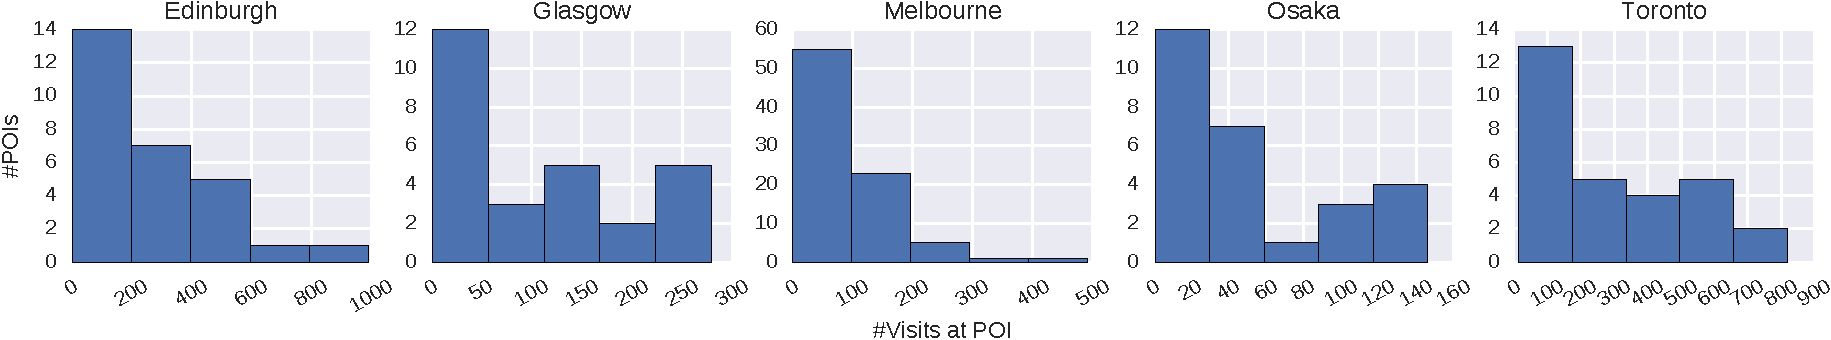
\includegraphics[width=\textwidth]{fig/poi_nvisit.pdf}
      \caption{Distribution of the number of visit at POI}
      \label{fig:nvisit}
      \end{figure*}
\item The distribution of POI visit duration is shown in figure \ref{fig:duration}.
      \begin{figure*}
      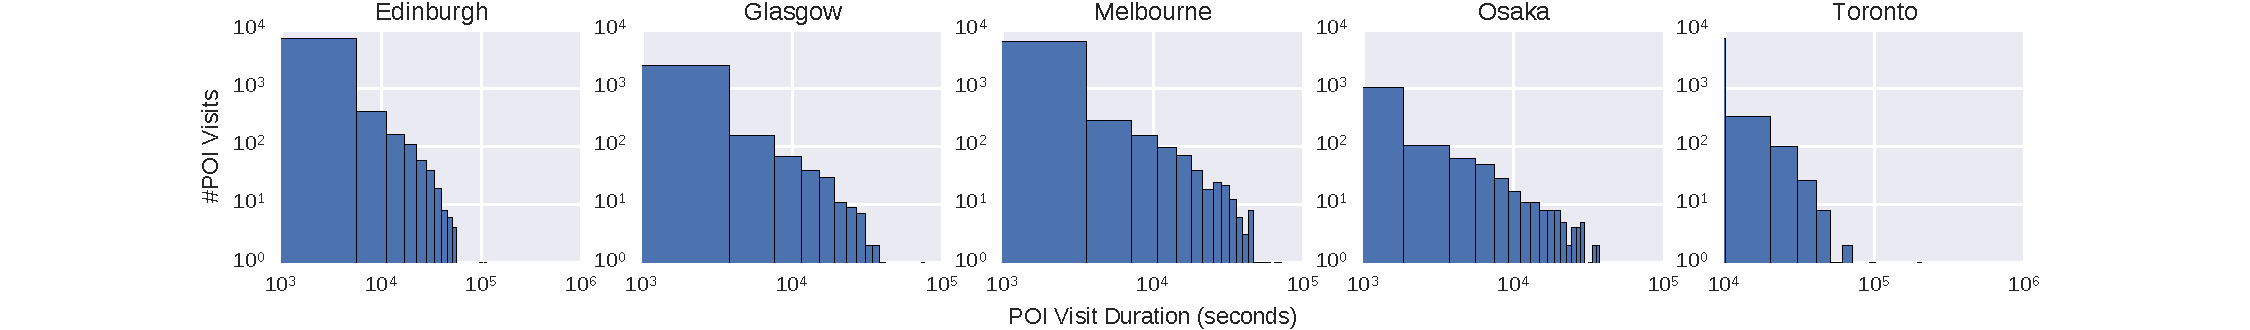
\includegraphics[width=\textwidth]{fig/visit_duration.pdf}
      \caption{Distribution of POI visit duration}
      \label{fig:duration}
      \end{figure*}
\item There are about $12$\% of trajectories in Melbourne dataset that were failed to be evaluated 
      using \textsc{PersTour} due to the timeout of integer programming solver, the timeout is $2$ hours.
\end{itemize}
